% =============================================================================
%  properties.figures.1.3.0.tex
%
%  Three TikZ figures supporting properties.1.3.0.md:
%
%    Figure 1 — State-transition diagram of Directory.tla.
%    Figure 2 — Proof-dependency DAG over T1–T6 and the helper lemma H.
%    Figure 3 — Hasse-style chain of the 9-step Predecessors ordering.
%
%  Compile with:  lualatex properties.figures.1.3.0.tex
%
%  Author. Jean-Gabriel Cordier, with Claude.
%  Kaizen step 1.3.0.
% =============================================================================

\documentclass[10pt,a4paper]{article}

\usepackage{fontspec}
\setmainfont{CMU Serif}
\setmonofont{CMU Typewriter Text}

\usepackage[a4paper,margin=2.2cm]{geometry}

\usepackage{tikz}
\usetikzlibrary{positioning,arrows.meta,fit,calc,shapes,shapes.geometric,shapes.misc,backgrounds,chains}

\usepackage{amsmath,amssymb}
\usepackage{microtype}
\usepackage{caption}
\captionsetup{font=small,labelfont=bf}

% ---- Reusable styles ---------------------------------------------------------

\tikzset{
  state/.style       = {draw, rounded corners=2pt, align=center,
                        minimum width=6.4cm, minimum height=0.85cm,
                        font=\small, inner sep=4pt},
  init/.style        = {state, fill=black!4},
  inter/.style       = {state, fill=blue!4},
  good/.style        = {state, fill=green!10, line width=0.7pt},
  bad/.style         = {state, fill=red!10,   line width=0.7pt},
  thm/.style         = {draw, rounded corners=3pt, fill=blue!5,
                        align=center, minimum width=1.7cm, minimum height=0.7cm,
                        font=\small\bfseries, inner sep=4pt},
  helper/.style      = {draw, rounded corners=3pt, fill=yellow!12,
                        align=center, minimum width=1.7cm, minimum height=0.7cm,
                        font=\small\itshape, inner sep=4pt},
  ext/.style         = {draw, dashed, rounded corners=3pt, fill=black!4,
                        align=center, font=\footnotesize, inner sep=4pt},
  hasse/.style       = {draw, rounded corners=2pt, fill=blue!3, align=center,
                        minimum width=4.4cm, minimum height=0.7cm,
                        font=\ttfamily\small, inner sep=3pt},
  edge/.style        = {-{Latex[length=2mm,width=1.6mm]}, line width=0.55pt},
  succ/.style        = {edge, draw=blue!55!black},
  fail/.style        = {edge, draw=red!60!black, dashed},
  dep/.style         = {edge, draw=black!75},
  caption_in/.style  = {font=\footnotesize\itshape, align=center}
}

% ---- Document ----------------------------------------------------------------

\begin{document}

\begin{center}
  {\Large\bfseries Properties — supporting figures}\\[2pt]
  \emph{kaizen step 1.3.0 \quad — \quad MarkdownToLaTeX 1.0.0}\\[6pt]
  Jean-Gabriel Cordier, with Claude
\end{center}

\bigskip

% =============================================================================
% Figure 1 — State-transition diagram
% =============================================================================

\section*{Figure 1 — State-transition diagram of \texttt{Directory.tla}}

The procedure threads a fixed chain of nine checks. From every
intermediate state, exactly two non-stutter transitions are enabled:
the (success) step that proves the next flag and advances along the
chain, and the (failure) step that latches \texttt{verdict := NOT\_MUST\_DO}.
The terminal state \texttt{MUST\_DO} is only reachable through the
ninth and final success.

\vspace{4pt}

\begin{center}
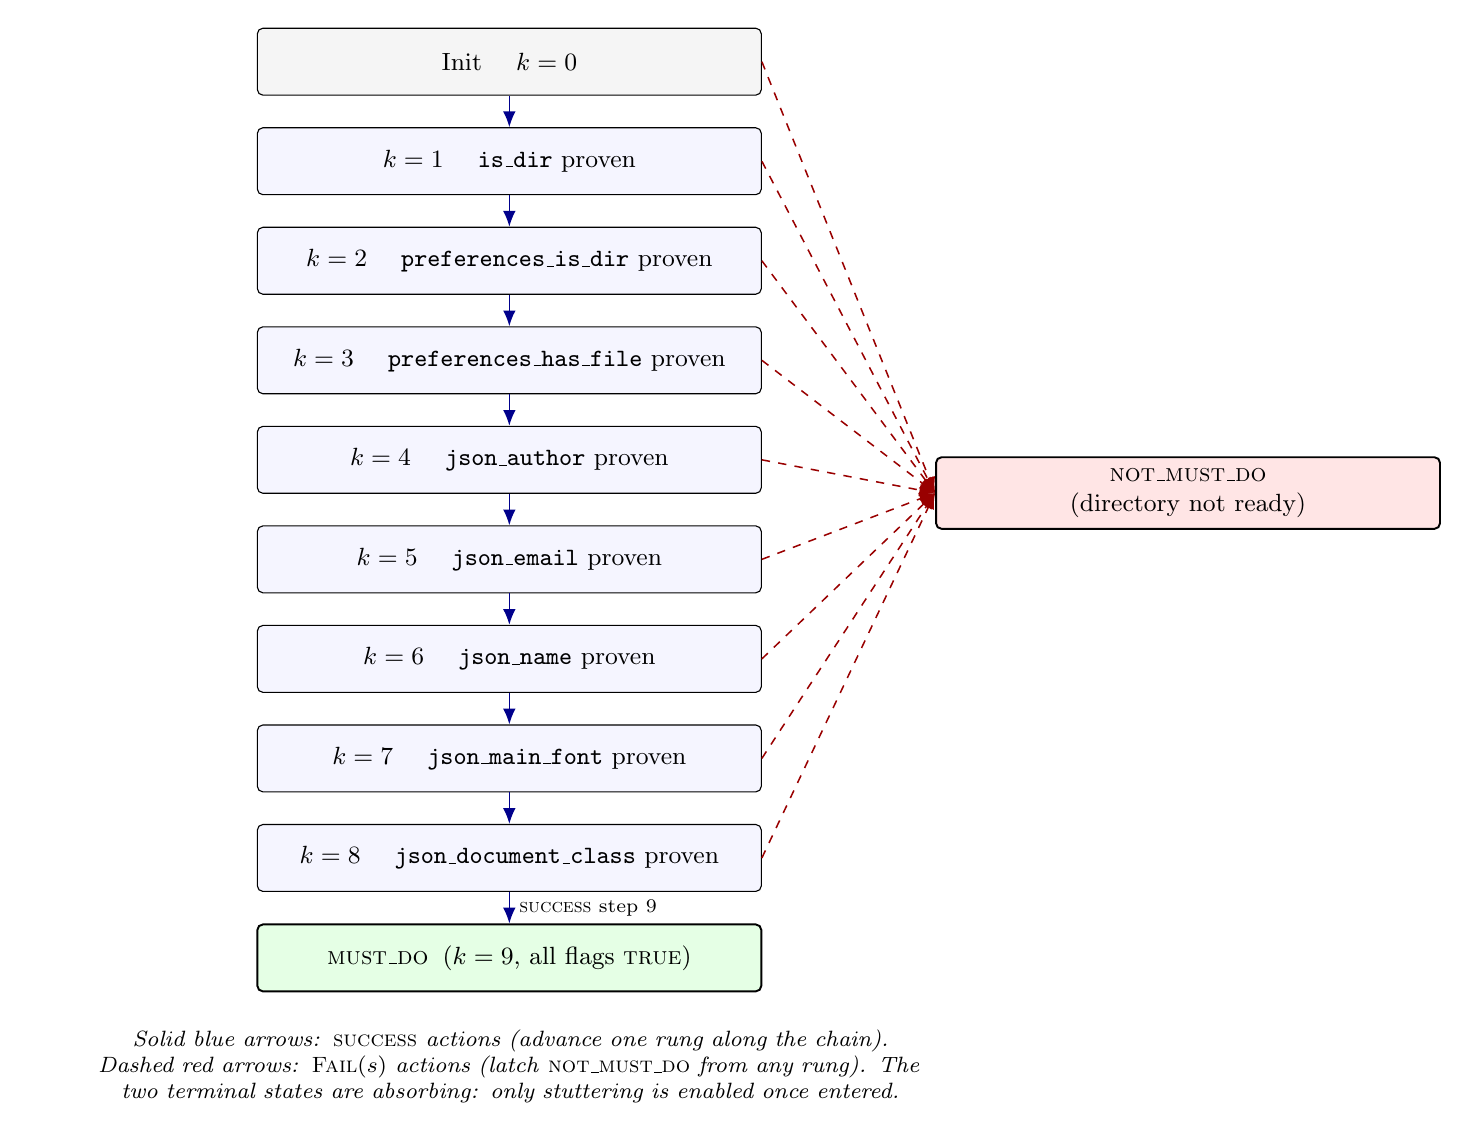
\begin{tikzpicture}[node distance=4mm and 22mm]

  % Vertical chain of intermediate states (Init + 8 intermediates).
  % S_k means "verdict = UNKNOWN, exactly k proof flags TRUE".
  \node[init]                   (S0) {Init \quad $k=0$};
  \node[inter, below=of S0]     (S1) {$k=1$ \quad \texttt{is\_dir} proven};
  \node[inter, below=of S1]     (S2) {$k=2$ \quad \texttt{preferences\_is\_dir} proven};
  \node[inter, below=of S2]     (S3) {$k=3$ \quad \texttt{preferences\_has\_file} proven};
  \node[inter, below=of S3]     (S4) {$k=4$ \quad \texttt{json\_author} proven};
  \node[inter, below=of S4]     (S5) {$k=5$ \quad \texttt{json\_email} proven};
  \node[inter, below=of S5]     (S6) {$k=6$ \quad \texttt{json\_name} proven};
  \node[inter, below=of S6]     (S7) {$k=7$ \quad \texttt{json\_main\_font} proven};
  \node[inter, below=of S7]     (S8) {$k=8$ \quad \texttt{json\_document\_class} proven};

  % Terminal MUST_DO at the bottom of the chain.
  \node[good,  below=of S8]     (MD) {\textsc{must\_do}\;\;($k=9$, all flags \textsc{true})};

  % NOT_MUST_DO as a single sink to the right; one Fail edge from every
  % intermediate state lands here.
  \node[bad, right=of S4, yshift=-12pt] (NMD) {\textsc{not\_must\_do}\\(directory not ready)};

  % Success edges along the chain.
  \draw[succ] (S0) -- (S1);
  \draw[succ] (S1) -- (S2);
  \draw[succ] (S2) -- (S3);
  \draw[succ] (S3) -- (S4);
  \draw[succ] (S4) -- (S5);
  \draw[succ] (S5) -- (S6);
  \draw[succ] (S6) -- (S7);
  \draw[succ] (S7) -- (S8);

  % Final success transition to MUST_DO.
  \draw[succ] (S8) -- (MD)
    node[midway, right, font=\scriptsize] {\textsc{success} step 9};

  % Failure edges: each intermediate state has a Fail(s) edge to NMD.
  \draw[fail] (S0.east) -- (NMD.west);
  \draw[fail] (S1.east) -- (NMD.west);
  \draw[fail] (S2.east) -- (NMD.west);
  \draw[fail] (S3.east) -- (NMD.west);
  \draw[fail] (S4.east) -- (NMD.west);
  \draw[fail] (S5.east) -- (NMD.west);
  \draw[fail] (S6.east) -- (NMD.west);
  \draw[fail] (S7.east) -- (NMD.west);
  \draw[fail] (S8.east) -- (NMD.west);

  % Legend.
  \node[caption_in, below=10pt of MD.south, anchor=north, text width=12cm] {
    Solid blue arrows: \textsc{success} actions (advance one rung along the chain).\quad
    Dashed red arrows: \textsc{Fail}$(s)$ actions (latch \textsc{not\_must\_do} from any
    rung). The two terminal states are absorbing: only stuttering is enabled
    once entered.
  };

\end{tikzpicture}
\end{center}

\vspace{2pt}

\noindent\textbf{Reading note.} Each state $S_k$ has \texttt{verdict =
"UNKNOWN"} and exactly $k$ proof flags set. The two terminal states
\textsc{must\_do} and \textsc{not\_must\_do} are absorbing: once entered, only
stuttering is enabled (theorem T2, verdict stability, in
\texttt{Directory.1.3.0.tla.txt}).

\clearpage

% =============================================================================
% Figure 2 — Proof-dependency DAG
% =============================================================================

\section*{Figure 2 — Proof-dependency DAG over T1–T6}

T1 (type-correctness) underpins every other proof in the module.
T2 (verdict stability) stands on its own — its proof depends only on
the action structure, not on TypeOK. The helper lemma H
(\texttt{ProvenAttemptedInvariant}) bridges proof flags and
\texttt{attempted}, and is consumed only by T6. T3 (termination) also
draws on the fairness clause $\mathrm{WF}_{\mathit{vars}}(\textit{Next})$
and on the leads-to chain of nine OMITTED links discharged
interactively in the TLA Toolbox.

\vspace{4pt}

\begin{center}
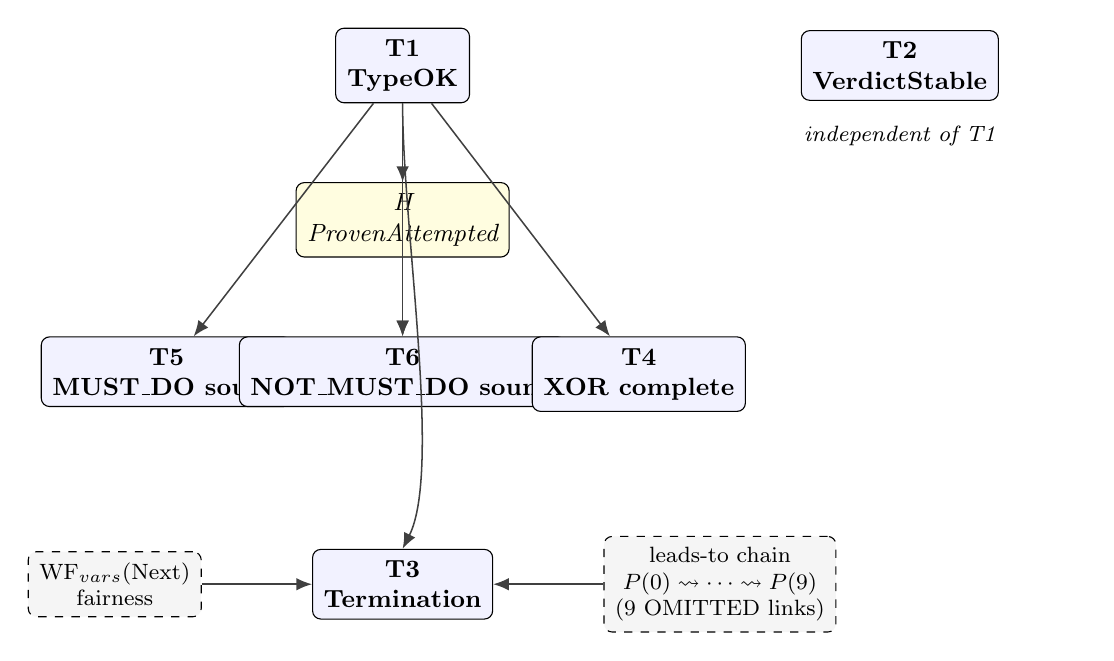
\begin{tikzpicture}[node distance=10mm and 18mm]

  % Tier 1: foundation
  \node[thm]                    (T1) {T1\\TypeOK};
  \node[thm, right=42mm of T1]  (T2) {T2\\VerdictStable};

  % Tier 2: helper
  \node[helper, below=of T1]    (H)  {H\\ProvenAttempted};

  % Tier 3: theorems built on T1 (and H)
  \node[thm, below=of H, xshift=-30mm] (T5) {T5\\MUST\_DO sound};
  \node[thm, below=of H]                (T6) {T6\\NOT\_MUST\_DO sound};
  \node[thm, below=of H, xshift=30mm]   (T4) {T4\\XOR complete};

  % Tier 4: liveness
  \node[thm, below=18mm of T6]  (T3) {T3\\Termination};

  % External inputs to T3
  \node[ext, left=14mm of T3]   (WF) {WF$_{vars}$(Next)\\fairness};
  \node[ext, right=14mm of T3]  (LT) {leads-to chain\\$P(0)\rightsquigarrow\dots\rightsquigarrow P(9)$\\(9 OMITTED links)};

  % Edges
  \draw[dep] (T1) -- (H);
  \draw[dep] (T1) -- (T5);
  \draw[dep] (T1) -- (T6);
  \draw[dep] (T1) -- (T4);
  \draw[dep] (T1.south) .. controls +(0,-1.6) and +(0.5,1) .. (T3.north);

  \draw[dep] (H)  -- (T6);

  \draw[dep] (WF) -- (T3);
  \draw[dep] (LT) -- (T3);

  % T2 is independent — show it visually
  \node[caption_in, below=2mm of T2.south, text width=4.5cm] {independent of T1};

\end{tikzpicture}
\end{center}

\vspace{2pt}

\noindent\textbf{Reading note.} Solid arrows are proof dependencies:
the head theorem is invoked in the body of the tail theorem's TLAPS
proof. Yellow node H is a helper lemma stated and proved in the same
module; dashed boxes on either side of T3 are external assumptions
(fairness from \texttt{Spec}, and the WF1 leads-to chain whose nine
links are flagged \texttt{OMITTED} in \texttt{Directory.1.3.0.tla.txt},
to be discharged in the TLA Toolbox).

\clearpage

% =============================================================================
% Figure 3 — Hasse-style chain of Predecessors
% =============================================================================

\section*{Figure 3 — Hasse-style chain of the \texttt{Predecessors} ordering}

The relation \texttt{Predecessors}$(s)$ is total: every step has every
earlier step as a strict predecessor and none as an incomparable peer.
The Hasse diagram is therefore a single linear chain. Step~9
(\texttt{json\_document\_class\_legal}) is the unique greatest element
and is also the only step whose success transitions \texttt{verdict} to
\texttt{MUST\_DO}.

\vspace{6pt}

\begin{center}
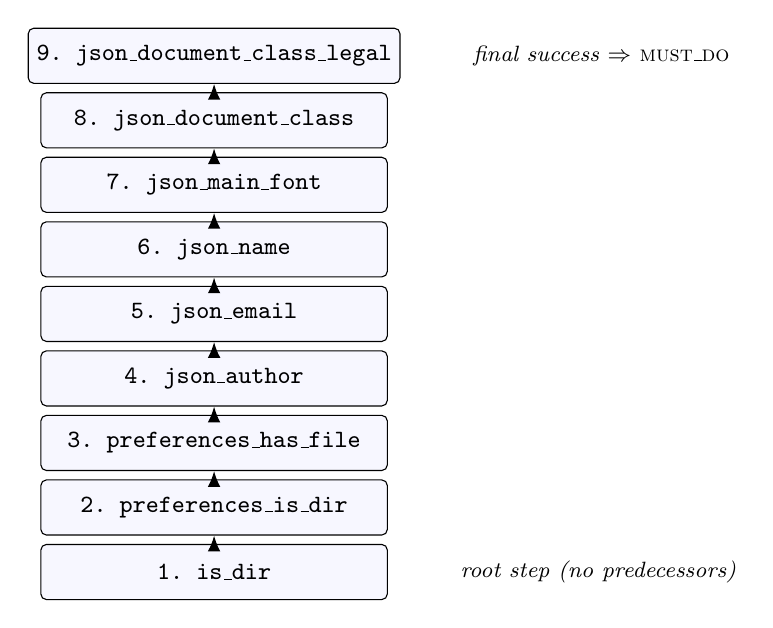
\begin{tikzpicture}[node distance=3pt and 0pt]
  \node[hasse]                (s9) {9.\ \texttt{json\_document\_class\_legal}};
  \node[hasse, below=of s9]   (s8) {8.\ \texttt{json\_document\_class}};
  \node[hasse, below=of s8]   (s7) {7.\ \texttt{json\_main\_font}};
  \node[hasse, below=of s7]   (s6) {6.\ \texttt{json\_name}};
  \node[hasse, below=of s6]   (s5) {5.\ \texttt{json\_email}};
  \node[hasse, below=of s5]   (s4) {4.\ \texttt{json\_author}};
  \node[hasse, below=of s4]   (s3) {3.\ \texttt{preferences\_has\_file}};
  \node[hasse, below=of s3]   (s2) {2.\ \texttt{preferences\_is\_dir}};
  \node[hasse, below=of s2]   (s1) {1.\ \texttt{is\_dir}};

  \draw[edge] (s1) -- (s2);
  \draw[edge] (s2) -- (s3);
  \draw[edge] (s3) -- (s4);
  \draw[edge] (s4) -- (s5);
  \draw[edge] (s5) -- (s6);
  \draw[edge] (s6) -- (s7);
  \draw[edge] (s7) -- (s8);
  \draw[edge] (s8) -- (s9);

  % Side annotations
  \node[caption_in, right=8mm of s9, anchor=west] {final success $\Rightarrow$ \textsc{must\_do}};
  \node[caption_in, right=8mm of s1, anchor=west] {root step (no predecessors)};
\end{tikzpicture}
\end{center}

\vspace{2pt}

\noindent\textbf{Reading note.} An arrow $a \to b$ means $a \in
\textit{Predecessors}(b)$. Read upward, this is also the temporal order
in which proof flags can flip from \textsc{false} to \textsc{true}: a
flag is provable only after every flag below it has already been proved.
This monotone chain is what makes the inductive arguments behind T5 and
T6 fall out cleanly.

\end{document}
